\documentclass[a4paper, 11pt]{article}

\usepackage{enumitem}
\usepackage{graphicx}
\usepackage{hyperref}
\usepackage[utf8]{inputenc}
\usepackage{minted}

\begin{document}

\title{
	\textbf{Queues in C}
}
\author{Neo Gullberg}
\date{Fall 2024}
\maketitle

\section{Introduction}
	For this assignment my task was to implement functionality for working with queues in the C programming language.
	A queue is a data structure that works on the \textit{first in, first out} (FIFO) principle,
	meaning the earliest element to arrive is the earliest one to leave, just like a queue in real life.
	The queue was implemented as a linked list.

\section{Implementation}
	Since we are implementing our queue as a linked list we need to have a struct to represent a cell of a linked list, which can be seen below:
	\begin{minted}[tabsize=4]{c}
typedef struct Cell Cell;
struct Cell
{
	int value;
	Cell *next;
};
	\end{minted}
	We also have the following struct to represent the queue itself. It stores a pointer to both the first and the last cell of the queue.
	This is because certain operations benefit from having either one and/or the other.
	From keeping track of both we introduce a few corner cases we have to take into consideration, but nothing too troublesome.
	\begin{minted}[tabsize=4]{c}
typedef struct
{
	Cell *first;
	Cell *last;
} Queue;
	\end{minted}

\section{Enqueue}
	Enqueue means to add an element to the end of a queue.
	The first method I wrote for this was the following:
	\begin{minted}[tabsize=4]{c}
void Queue_enqueue(Queue *queue, int value)
{
	if (queue == NULL) return;

	Cell **current = &queue->first;

	while (*current != NULL)
	{
		current = &(*current)->next;
	}

	*current = Cell_construct(value);
}
	\end{minted}
	This method actually does not make use of the pointer to the last element, since I wrote this before I added that (which is also the reason why we do not update it).
	Since this method only makes us of the pointer to the first element, we have to traverse all cells until we find the last one and then create a new one and add that.
	\begin{figure}[H]
		\centering
		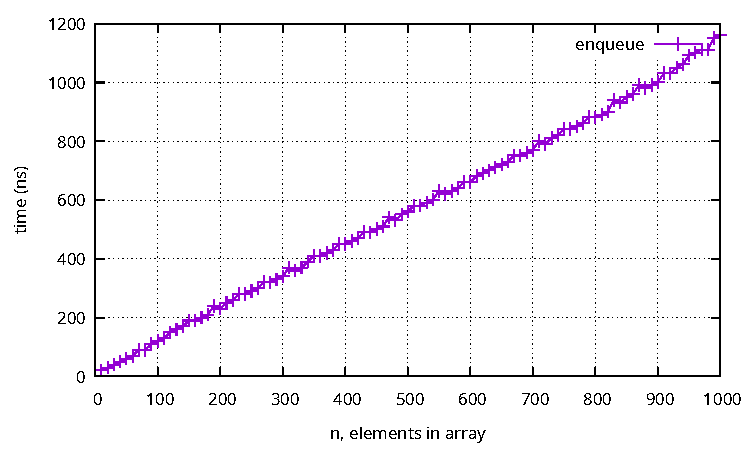
\includegraphics[scale=0.8]{graphs/enqueue.pdf}
		\caption{
			Graph showing the time it took to add an element to the end of a queue of size \(n\) if we only have access to the first element.
		}
	\end{figure}
	Expectedly this graph shows that the operation has a time complexity of \(O(n)\),
	since we have to traverse \(n\) number of elements to add an element to the end of a queue of size \(n\).

\section{Enqueue Optimized}
	This is how I implemented the method using the fact we could instantly access the last element in the queue.
	\begin{minted}[tabsize=4]{c}
void Queue_enqueue_optimized(Queue *queue, int value)
{
	if (queue == NULL) return;

	Cell *new = Cell_construct(value);

	if (queue->last == NULL)
		queue->first = new;
	else
		queue->last->next = new;

	queue->last = new;
}
	\end{minted}
	It is quite straightforward.
	However, we have to take into consideration whether or not the queue is empty or not.
	Therefore, it splits into two cases.
	If there is no last element (i.e. the queue is empty) we set the first and last element to be the new element.
	Otherwise we set the old last element to point to the new element, and then set the last element pointer to point to the new one.
	Notice that there is no looping going on in this implementation, opposed to the last one.
	\begin{figure}[H]
		\centering
		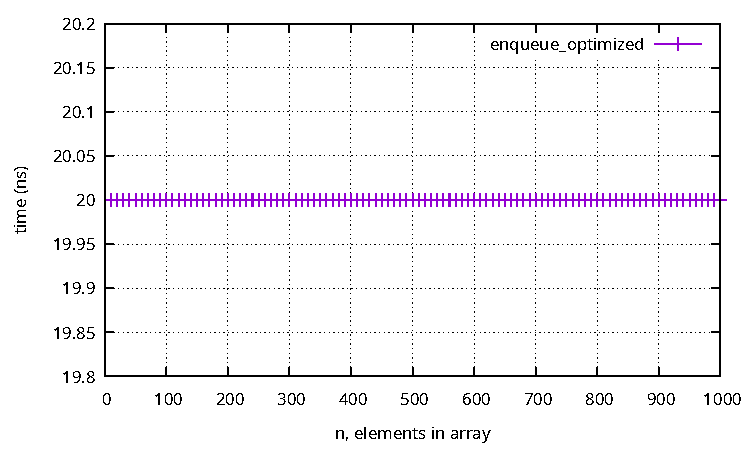
\includegraphics[scale=0.8]{graphs/enqueue_optimized.pdf}
		\caption{
			Graph showing the time it took to add an element to the end of a queue of size \(n\) if we have access to the last element.
		}
	\end{figure}
	This time the time complexity is \(O(1)\) which is a great improvement down from \(O(n)\).

\section{Dequeue}
	Lastly we have the dequeue operation which is the opposite of enqueue, namely it removes an element.
	\begin{minted}[tabsize=4]{c}
dequeue_result Queue_dequeue(Queue *queue)
{
	dequeue_result result = {
		0,
		false
	};

	if (queue != NULL && queue->first != NULL)
	{
		result.value = queue->first->value;
		result.valid = true;

		Cell *to_remove = queue->first;
		queue->first = to_remove->next;
		Cell_destruct(to_remove);
		if (queue->first == NULL)
		{
			queue->last = NULL;
		}
	}

	return result;
}
	\end{minted}
	It returns a struct named \texttt{dequeue\_result} which holds a value and a flag which specifies whether or not the result is valid or not.
	If the queue is a \texttt{NULL} pointer, or empty, no value is able to be retrieved.
	In that case the valid flag is false, otherwise it is true.
	This implementation does not necessarily make use of the pointer we have to the last element,
	but it does take it into consideration.
	If we call this when there is only one element in the queue we have to make sure to change the last pointer to point to a \texttt{NULL} reference
	(since there will no longer be a last element).
	\begin{figure}[H]
		\centering
		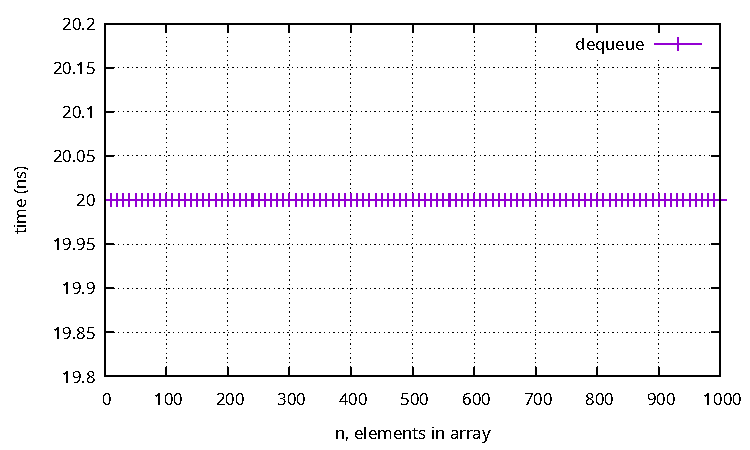
\includegraphics[scale=0.8]{graphs/dequeue.pdf}
		\caption{
			Graph showing the time it took to remove an element from the end of a queue of size \(n\).
		}
	\end{figure}
	The graph shows a time complexity of \(O(n)\), which is to be expected since we do not have to perform any looping.

\section{Source Code}
	If anyone is interested, the source code for this project can be found over at:
	\url{https://github.com/neogulgul/ID1021/tree/main/queue}

\end{document}
